\section{Actividades y Metodología}

%Localización física y ubicación de instalaciones:

El proyecto se llevó a cabo en la Facultad de Ingeniería de la Universidad Nacional de La Plata (UNLP).
Los ensayos necesarios se realizaron en el Área Técnica de Electrónica e Instrumental (ATEI) del Departamento de Electrotecnia.
Se realizaron consultas semanales con el tutor para el seguimiento del desarrollo del proyecto y
revisión de las decisiones tomadas por el equipo de trabajo.

Para alcanzar las metas y los objetivos propuestos, se llevaron a cabo las siguientes actividades:

\subsection{Estudio de bibliografía y diseño} \label{subsection:estudio_bibliografia}

En base a los requerimientos del proyecto y con el objetivo de capacitarse, se estudiaron y analizaron aspectos de seguridad, 
curvas de carga de la batería y topologías de convertidores de potencia. 
Se evaluaron las diferentes alternativas posibles y, en base a su complejidad y a su costo,
se eligió la solución más adecuada para el logro de los objetivos. 

Se realizaron simulaciones en SPICE (programa de simulación con énfasis en circuitos integrados),
separando el proceso en 4 partes:
\begin{itemize}
    \item Fuente conmutada: Convierte la tensión alterna de la red doméstica en una tensión continua.
    \item Fuente de corriente: Brinda una corriente constante a la batería durante la primera etapa de carga.
    \item Circuito de control: Alterna entre las etapas de carga.
\end{itemize}

En la Figura \ref{fig:esquema_cargador} se puede observar el esquema en bloques del cargador.
El circuito de la fuente conmutada está compuesto por los bloques de rectificación, filtrado y conversión DC-DC.
El controlador se encarga de generar una señal PWM en base a la tensión y la corriente de la batería.
La referencia es una señal de corriente ya que la tensión nominal del cargador es fija.

Para disminuir las pérdidas de potencia en la etapa de corriente constante y obtener una mayor eficiencia, se modificó la estructura del cargador con respecto al diseño original. 
En primera instancia, para mantener la tensión a la salida del convertidor en 42V, se propuso un ciclo de trabajo constante 
con el cual la caída de tensión en la etapa de control de corriente generaba una disipación de potencia excesiva.
Modificando el circuito de conversión que controla tanto la corriente como la tensión se evita una etapa posterior limitadora de corriente.

%incluir esquema de cargador
\begin{figure}
    \centering
    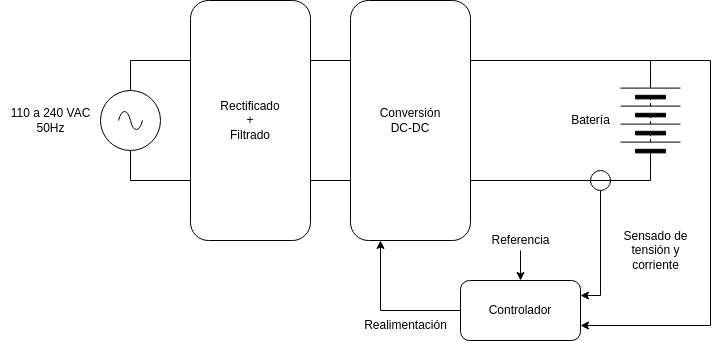
\includegraphics[width=\textwidth]{images/esquema_cargador_v2.png}
    \caption{Esquema del cargador}
    \label{fig:esquema_cargador}
\end{figure}

\subsection{Simulaciones}
Con el fin de verificar el diseño el circuito fue diseñado y probado en LTspice \cite{ltspice}.
El proceso se dividió en las siguientes etapas:
\begin{enumerate}
    \item Simulación del rectificador de entrada
    \item Simulación del convertidor
    \item Simulación del driver para el MOSFET high-side
    \item Simulación del circuito de control
    \item Simulación de distintos modelos de batería
\end{enumerate}

\subsection{Implementación y validación}
Se construyó un prototipo del cargador, realizando una primera versión con una placa perforada
y luego diseñando un circuito impreso para la implementación final.
Finalmente, operando a lazo abierto con un ciclo de trabajo fijo, se realizaron mediciones de tensión y corriente sobre los elementos con
con el fin de validar los resultados obtenidos en las simulaciones.